\clearpage
\section*{LAMPIRAN A Term of References}
\addcontentsline{toc}{chapter}{Lampiran A. \textit{Term of References} (TOR)}
\label{app:tor}

\begin{framed}
\begin{center}
{\bfseries\Large TERM OF REFERENCES}\\[4pt]
{\bfseries Pengujian Perangkat Lunak (\textit{Quality Assurance}) Aplikasi Komatsu ESS}\\[2pt]
PT Radya Anugrah Digital
\end{center}

\begin{enumerate}[label=\arabic*.,leftmargin=1.2cm,itemsep=6pt]

\item \textbf{TUJUAN PEKERJAAN}

PT Radya Anugrah Digital (Radyalabs) mengembangkan aplikasi Komatsu ESS untuk klien, yaitu Komatsu. Agar aplikasi tersebut berfungsi sesuai kebutuhan klien dan bebas dari \textit{bug} yang berarti sebelum diserahkan, diperlukan kegiatan pengujian yang terencana. Tujuan pekerjaan ini adalah memastikan kualitas aplikasi Komatsu ESS melalui kegiatan \textit{Quality Assurance} (QA), yaitu penyusunan \textit{test script}, \textit{module testing}, \textit{integration testing}, dan \textit{regression testing}, disertai pelaporan \textit{bug} . Pekerjaan ini dilaksanakan oleh dua mahasiswa KP yang sama-sama berperan sebagai \textit{Quality Assurance}. Hasil pekerjaan diperuntukkan bagi tim \textit{developer} Radyalabs dan, melalui tim tersebut, bagi Komatsu sebagai pengguna akhir.

\item \textbf{LINGKUP PEKERJAAN}

Lingkup pekerjaan tim QA pada proyek Komatsu ESS mencakup:
\begin{enumerate}[label=\arabic*)]
\item analisis kebutuhan dan spesifikasi fitur sebagai dasar pengujian;
\item penyusunan draf \textit{test script};
\item \textit{module testing};
\item \textit{integration testing};
\item \textit{regression testing} setelah perbaikan atau perubahan fitur;
\item pelaporan dan \textit{bug tracking} hingga tuntas; dan
\item pendokumentasian hasil pengujian.
\end{enumerate}
Bagian yang dikerjakan mahasiswa KP adalah pengujian modul-modul yang ditugaskan oleh pembimbing kepada masing-masing mahasiswa, dengan rincian yang ditetapkan pembimbing selama KP berlangsung.

\item \textbf{HASIL PEKERJAAN}

Hasil pekerjaan yang diharapkan adalah:
\begin{enumerate}[label=\arabic*)]
\item \textit{test script} untuk modul yang ditugaskan;
\item \textit{bug report} yang memuat \textit{steps to reproduce}, \textit{expected result}, \textit{actual result}, \textit{severity}, dan bukti (\textit{screenshot} atau rekaman);
\item laporan hasil \textit{module testing}, antarmodul, dan regresi; dan
\item aplikasi Komatsu ESS yang kualitasnya meningkat karena \textit{bug} yang ditemukan telah diperbaiki oleh tim \textit{developer}.
\end{enumerate}

\item \textbf{BATASAN}

\begin{enumerate}[label=\arabic*)]
\item Pekerjaan mahasiswa dibatasi pada kegiatan pengujian. Perbaikan \textit{bug} pada \textit{source code} menjadi tanggung jawab tim \textit{developer}.
\item Pengujian dilakukan pada lingkungan \textit{staging} dan bukan pada lingkungan produksi milik klien.
\item Mahasiswa hanya mengakses fitur, data, dan dokumen proyek sesuai izin yang diberikan pembimbing.
\item Seluruh informasi proyek dan data klien bersifat rahasia dan tidak boleh disebarluaskan. Isi laporan KP yang memuat informasi proyek harus mendapat persetujuan pembimbing.
\item Spesifikasi perangkat yang digunakan mengikuti ketentuan pada butir Lingkungan Pengembangan.
\end{enumerate}

\item \textbf{ASUMSI}

\begin{enumerate}[label=\arabic*)]
\item Dokumen kebutuhan atau spesifikasi fitur tersedia dan dapat diakses oleh mahasiswa.
\item Lingkungan pengujian, akun uji, dan data uji disediakan oleh perusahaan.
\item \textit{Build} aplikasi yang akan diuji tersedia sesuai jadwal rilis tim \textit{developer}.
\item Pembimbing dan tim \textit{developer} tersedia untuk klarifikasi kebutuhan dan pembahasan \textit{bug}.
\item Ketergantungan pada jadwal pengembangan dan perubahan kebutuhan dari klien dapat menggeser jadwal pengujian.
\end{enumerate}

\Needspace{10\baselineskip}
\item \textbf{METODOLOGI PEKERJAAN}

Pekerjaan dilaksanakan dengan siklus pengujian perangkat lunak yang berjalan beriringan dengan iterasi pengembangan aplikasi. Pengujian dilakukan secara bertahap dari cakupan kecil ke cakupan luas, yaitu dari modul, lalu antarmodul, lalu regresi. Tahapan tersebut dipetakan pada Tabel~A.1. Pelaporan \textit{bug} dilakukan di setiap tahap pengujian.

\begin{center}
\textbf{Tabel A.1} Pemetaan metodologi ke dalam tahapan pekerjaan\\[4pt]
\small
\begin{tabularx}{\linewidth}{|c|p{2.9cm}|X|p{2.6cm}|}
\hline
\textbf{No.} & \textbf{Tahap} & \textbf{Kegiatan} & \textbf{Hasil Antara} \\
\hline
1 & Orientasi & Mempelajari aplikasi, alur bisnis, alat kerja, dan prosedur tim & Pemahaman sistem \\
\hline
2 & Penyusunan draf \textit{test script} & Menganalisis \textit{requirement} fitur dan menyusun \textit{test script} tiap modul & \textit{Test script} \\
\hline
3 & \textit{Module testing} & Menjalankan \textit{test script} pada masing-masing modul dan melaporkan \textit{bug} & Hasil uji modul dan \textit{bug report} \\
\hline
4 & \textit{Integration testing} & Menguji alur yang melibatkan lebih dari satu modul dan interaksi antarmodul & Hasil uji antarmodul dan \textit{bug report} \\
\hline
5 & \textit{Regression testing} & Menjalankan ulang pengujian untuk memverifikasi perbaikan dan memastikan fitur lain tidak terdampak & Hasil verifikasi \\
\hline
6 & Dokumentasi & Merangkum hasil pengujian dan menyusun laporan KP & Laporan hasil uji dan laporan KP \\
\hline
\end{tabularx}
\end{center}

\item \textbf{LINGKUNGAN PENGEMBANGAN}

\begin{enumerate}[label=\arabic*)]
\item Perangkat keras: komputer atau laptop kerja dan perangkat uji (\textit{smartphone}) sesuai kebutuhan pengujian.
\item Perangkat lunak: aplikasi Komatsu ESS pada lingkungan \textit{staging}, peramban web, \textit{bug tracker} dan alat manajemen tugas yang digunakan tim, alat dokumentasi \textit{test case}, serta alat komunikasi tim.
\end{enumerate}
Rincian versi dan alat mengikuti yang digunakan oleh tim proyek.

\Needspace{12\baselineskip}
\item \textbf{JADWAL}

Kerja praktik dilaksanakan pada 22 Juni 2026 sampai dengan 22 September 2026 (13 minggu) di Bandung. Rencana kegiatan ditunjukkan pada Gambar~A.1.

\begin{center}
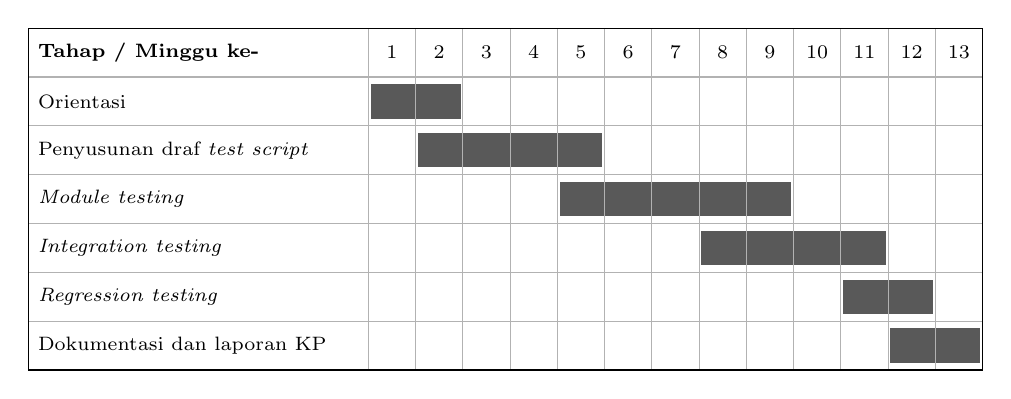
\begin{tikzpicture}[x=0.6cm,y=0.62cm,font=\scriptsize]
\def\labw{7.2}
% kepala kolom minggu
\foreach \w in {1,...,13}{
  \node at (\w-0.5,0.5) {\w};
}
\node[anchor=west] at (-\labw,0.5) {\textbf{Tahap / Minggu ke-}};
% baris tahap: nama, awal, akhir
\foreach \name/\a/\b [count=\r from 1] in {%
  Orientasi/1/2,%
  Penyusunan draf \textit{test script}/2/5,%
  \textit{Module testing}/5/9,%
  \textit{Integration testing}/8/11,%
  \textit{Regression testing}/11/12,%
  Dokumentasi dan laporan KP/12/13}{
  \node[anchor=west] at (-\labw,-\r+0.5) {\name};
  \fill[black!65] (\a-1+0.05,-\r+0.15) rectangle (\b-0.05,-\r+0.85);
}
% grid
\foreach \w in {0,...,13}{\draw[black!30] (\w,1) -- (\w,-6);}
\foreach \r in {0,...,6}{\draw[black!30] (-\labw,1-\r-0) -- (13,1-\r-0);}
\draw (-\labw,1) rectangle (13,-6);
\end{tikzpicture}
\\[4pt]\textbf{Gambar A.1} \textit{Gantt chart} rencana pelaksanaan pekerjaan
\end{center}

\item \textbf{PENUGASAN STAF}

Pekerjaan dilakukan oleh dua mahasiswa dengan peran yang sama, yaitu \textit{Quality Assurance}, di bawah arahan pembimbing instansi. Seluruh tahapan pada butir Metodologi Pekerjaan dijalani oleh kedua mahasiswa. Perbedaannya terletak pada modul yang diuji, yang dibagi oleh pembimbing dan dibagi secara merata di antara keduanya. \textit{Integration testing} dilakukan bersama untuk alur yang melibatkan modul dari kedua mahasiswa.

\begin{center}
\small
\begin{tabularx}{\linewidth}{|p{3.6cm}|p{2.6cm}|X|}
\hline
\textbf{Nama} & \textbf{Peran} & \textbf{Tanggung Jawab} \\
\hline
Naufarrel Zhafif Abhista (13523149) & \textit{Quality Assurance} & Menyusun \textit{test script}, menguji, dan melaporkan \textit{bug} pada modul yang ditugaskan; \textit{integration testing} dan regresi bersama \\
\hline
Zulfaqqar Nayaka Athadiansyah (13523094) & \textit{Quality Assurance} & Menyusun \textit{test script}, menguji, dan melaporkan \textit{bug} pada modul yang ditugaskan; \textit{integration testing} dan regresi bersama \\
\hline
\end{tabularx}
\end{center}

\Needspace{50\baselineskip}
\item \textbf{MEKANISME PENGENDALIAN DAN PEMANTAUAN}

\begin{enumerate}[label=\arabic*)]
\item Setiap mahasiswa mencatat kegiatan hariannya pada \textit{log activity} masing-masing dan menyampaikannya kepada pembimbing.
\item Kemajuan pengujian dilaporkan secara lisan kepada pembimbing dan tim proyek melalui pertemuan rutin, dari mahasiswa kepada pembimbing instansi.
\item \textit{Bug} dilaporkan melalui \textit{bug tracker} yang digunakan tim dan dibahas bersama tim \textit{developer}.
\item Pembimbing instansi memberikan umpan balik dan penilaian akhir pada akhir KP.
\end{enumerate}

Tonggak (\textit{milestone}) pekerjaan ditunjukkan pada Tabel~A.2.

\begin{center}
\textbf{Tabel A.2} \textit{Milestone} pelaksanaan pekerjaan\\[4pt]
\small
\begin{tabularx}{\linewidth}{|c|X|p{3.3cm}|}
\hline
\textbf{No.} & \textbf{Milestone} & \textbf{Perkiraan Waktu} \\
\hline
1 & Orientasi selesai dan penyusunan \textit{test script} dimulai & Minggu 2 \\
\hline
2 & Draf \textit{test script} selesai dan \textit{module testing} dimulai & Minggu 5 \\
\hline
3 & \textit{Integration testing} dimulai & Minggu 8 \\
\hline
4 & \textit{Regression testing} dimulai & Minggu 11 \\
\hline
5 & Seluruh pengujian selesai dan draf laporan KP diserahkan kepada pembimbing & Minggu 12 \\
\hline
6 & Penilaian dan pengesahan laporan oleh pembimbing & Minggu 13 \\
\hline
\end{tabularx}
\end{center}

\Needspace{10\baselineskip}
\item \textbf{MANAJEMEN RESIKO}

\begin{center}
\small
\begin{tabularx}{\linewidth}{|p{3.6cm}|p{1.5cm}|X|}
\hline
\textbf{Risiko} & \textbf{Prioritas} & \textbf{Pengendalian} \\
\hline
Perubahan \textit{requirement} dari klien & Tinggi & Memperbarui \textit{test script} dan berkoordinasi dengan pembimbing \\
\hline
\textit{Build} terlambat atau tidak stabil & Tinggi & Menyesuaikan urutan pengujian dan mengerjakan \textit{test script} atau dokumentasi terlebih dahulu \\
\hline
Lingkungan atau data uji tidak tersedia & Sedang & Meminta dukungan tim \textit{developer} lebih awal \\
\hline
Pemahaman domain bisnis kurang & Sedang & Bertanya kepada pembimbing dan mempelajari dokumen proyek \\
\hline
\end{tabularx}
\end{center}

\item \textbf{LAIN-LAIN}

\begin{enumerate}[label=\arabic*)]
\item Kedua mahasiswa menaati tata tertib, jam kerja, dan ketentuan kerahasiaan perusahaan.
\item Hasil pekerjaan menjadi milik perusahaan, sedangkan mahasiswa berhak menggunakan pengalaman kerja untuk keperluan laporan KP dengan persetujuan pembimbing.
\end{enumerate}
\end{enumerate}

\Needspace{20\baselineskip}
\vspace{0.6cm}
\begin{center}
Bandung, 23 Juni 2026

\vspace{0.3cm}
Disetujui oleh,

\vspace{0.4cm}
Pembimbing Instansi

\vspace{1.6cm}
\textbf{Alyssa Christella}\\
\textit{Project Manager} dan \textit{Mentor}\\
PT Radya Anugrah Digital

\vspace{0.6cm}
Mahasiswa Kerja Praktik

\vspace{0.4cm}
\begin{minipage}[t]{0.48\linewidth}
\centering

\includegraphics[height=1.53cm,trim=200 410 250 300,clip]{figures/ttd-naufarrel.png}\\
\textbf{Naufarrel Zhafif Abhista}\\
NIM 13523149
\end{minipage}\hfill
\begin{minipage}[t]{0.48\linewidth}
\centering

\includegraphics[height=1.53cm,trim=15 10 0 10,clip]{figures/ttd-nayaka.png}\\
\textbf{Zulfaqqar Nayaka Athadiansyah}\\
NIM 13523094
\end{minipage}
\end{center}
\end{framed}

\clearpage
